
\chapter{Complete Experimental Results}
\label{app:full_results}

Table~\ref{tab:features} lists the 19 features retained from the ToN\_IoT dataset after removing constant and identifier columns.

\begin{table}[ht]
    \centering
    \small
    \begin{tabular}{llp{7.5cm}}
        \toprule
        \textbf{Feature} & \textbf{Type} & \textbf{Description} \\
        \midrule
        src\_port, dst\_port  & Numerical & Source and destination transport port numbers \\
        proto                & Binary    & Transport protocol (TCP\,=\,0, UDP\,=\,1) \\
        service              & Categorical & Application service (none, DNS, HTTP, SSL) \\
        duration             & Numerical & Flow duration in seconds \\
        src\_bytes, dst\_bytes & Numerical & Bytes sent by source / destination \\
        conn\_state           & Categorical & TCP connection state (REJ, S0, SF, etc.) \\
        src\_pkts, dst\_pkts   & Numerical & Packets sent by source / destination \\
        src\_ip\_bytes, dst\_ip\_bytes & Numerical & IP-level bytes (including headers) \\
        dns\_qclass, dns\_qtype, dns\_rcode & Numerical & DNS query class, type, and response code \\
        dns\_AA, dns\_RD, dns\_RA, dns\_rejected & Binary & DNS flags (authoritative, recursion, etc.) \\
        \bottomrule
    \end{tabular}
    \caption{The 19 features retained after removing constant and identifier columns.}
    \label{tab:features}
\end{table}

Table~\ref{tab:full_results} consolidates all experimental results across models, tasks, and dataset sizes --- including the autoencoder for completeness. Classical supervised models use the full balanced training set. The autoencoder uses the full ${\sim}28{,}000$ normal samples and is averaged over 10~seeds. Quantum results at $n=500$ are mean~$\pm$~std over 10~seeds; other quantum sizes use seed~42 only.

\begin{table}[ht]
\centering
\small
\begin{tabular}{llcccc}
    \toprule
    \textbf{Model} & \textbf{Task} & $n=100$ & $n=250$ & $n=500$ & $n=1000$ \\
    \midrule
    \multicolumn{6}{l}{\textit{Classical supervised --- full training set (accuracy)}} \\
    \midrule
    Random Forest   & Standard  & \multicolumn{4}{c}{0.990} \\
    SVM (RBF)       & Standard  & \multicolumn{4}{c}{0.970} \\
    NN-Medium       & Standard  & \multicolumn{4}{c}{0.960} \\
    NN-Small        & Standard  & \multicolumn{4}{c}{0.925} \\
    \midrule
    NN-Small        & Zero-day  & \multicolumn{4}{c}{0.028} \\
    SVM (RBF)       & Zero-day  & \multicolumn{4}{c}{0.024} \\
    NN-Medium       & Zero-day  & \multicolumn{4}{c}{0.017} \\
    Random Forest   & Zero-day  & \multicolumn{4}{c}{0.003} \\
    \midrule
    \multicolumn{6}{l}{\textit{Classical unsupervised --- Autoencoder, ${\sim}28{,}000$ normal samples, 10 seeds (detection rate)}} \\
    \midrule
    Autoencoder     & Zero-day  & \multicolumn{4}{c}{\textbf{0.705 $\pm$ 0.144}} \\
    \midrule
    \multicolumn{6}{l}{\textit{Quantum --- Standard task, training subsamples of size $n$ (accuracy)}} \\
    \midrule
    Re-uploading 1q & Standard  & 0.750 & 0.730 & 0.752 $\pm$ 0.039 & 0.730 \\
    Re-uploading 4q & Standard  & 0.695 & 0.700 & 0.692 $\pm$ 0.011 & 0.700 \\
    QCNN (8q)       & Standard  & 0.705 & 0.695 & 0.679 $\pm$ 0.025 & 0.680 \\
    \midrule
    \multicolumn{6}{l}{\textit{Quantum --- Zero-day task, training subsamples of size $n$ (detection rate)}} \\
    \midrule
    QCNN (8q)       & Zero-day  & 0.005 & 0.020 & \textbf{0.490 $\pm$ 0.305} & 0.010 \\
    Re-uploading 1q & Zero-day  & 0.060 & 0.170 & 0.092 $\pm$ 0.036 & 0.105 \\
    Re-uploading 4q & Zero-day  & 0.040 & 0.040 & 0.075 $\pm$ 0.023 & 0.080 \\
    \bottomrule
\end{tabular}
\caption{Consolidated results across all models, tasks, and training-set sizes. \textbf{Classical supervised} models are trained on the full balanced training set and reported as single numbers. \textbf{The autoencoder} uses all ${\sim}28{,}000$ normal samples, is tested on the full 7,034-sample injection set, and is averaged over 10 seeds. \textbf{Quantum} models use subsamples of size $n$ (stratified for standard, fixed random for zero-day); $n=500$ results are mean $\pm$ std over 10 seeds, other sizes use seed~42 only. The QCNN zero-day values at $n\neq 500$ use seed~42, which lands in a barren plateau --- the multi-seed run at $n=500$ shows that 7/10 seeds actually achieve 54--76\% detection (mean 68.6\% $\pm$ 6.8\% excluding the 3 collapsed seeds).}
\label{tab:full_results}
\end{table}

The complete per-seed breakdown for the QCNN over 10~seeds is given in Table~\ref{tab:res_seeds} of Section~\ref{sec:res_sensitivity}. Re-uploading per-seed values are tightly clustered around their means (standard deviations of 0.039 and 0.011 on the standard task; 0.036 and 0.023 on zero-day) and are not reported individually.

% ---- Confusion Matrices ----

\section{Confusion Matrices}
\label{app:confusion}

Table~\ref{tab:cm_std_annex} shows confusion matrices for the best classical model (Random Forest) and the best quantum model (QCNN, seed~0) on the standard 3-class task. Table~\ref{tab:cm_zd_annex} shows the zero-day confusion matrices.

\begin{table}[ht]
\centering
\small
\begin{tabular}{c|ccc}
    \multicolumn{4}{c}{\textbf{Random Forest} --- Accuracy 0.990} \\
    \toprule
     & \textbf{pred.\ DoS} & \textbf{pred.\ Inj.} & \textbf{pred.\ Norm.} \\
    \midrule
    \textbf{DoS}    & 65 &  0 &  1 \\
    \textbf{Inj.}   &  0 & 67 &  0 \\
    \textbf{Norm.}   &  0 &  1 & 66 \\
    \bottomrule
\end{tabular}
\hspace{0.8cm}
\begin{tabular}{c|ccc}
    \multicolumn{4}{c}{\textbf{QCNN (seed 0)} --- Accuracy 0.720} \\
    \toprule
     & \textbf{pred.\ DoS} & \textbf{pred.\ Inj.} & \textbf{pred.\ Norm.} \\
    \midrule
    \textbf{DoS}    & 64 &  0 &  2 \\
    \textbf{Inj.}   &  0 & 64 &  3 \\
    \textbf{Norm.}   & 43 &  8 & 16 \\
    \bottomrule
\end{tabular}
\caption{Standard 3-class confusion matrices. The Random Forest achieves near-perfect separation. The QCNN correctly classifies DoS and injection but struggles with normal traffic, misclassifying 43 out of 67 normal samples as DoS.}
\label{tab:cm_std_annex}
\end{table}

\begin{table}[ht]
\centering
\small
\begin{tabular}{c|cc}
    \multicolumn{3}{c}{\textbf{QCNN (seed 0)} --- Zero-day Acc.\ 0.755} \\
    \toprule
     & \textbf{pred.\ Normal} & \textbf{pred.\ Attack} \\
    \midrule
    \textbf{Injection}  & 49 & 151 \\
    \bottomrule
\end{tabular}
\hspace{0.8cm}
\begin{tabular}{c|cc}
    \multicolumn{3}{c}{\textbf{Random Forest} --- Zero-day Acc.\ 0.003} \\
    \toprule
     & \textbf{pred.\ Normal} & \textbf{pred.\ Attack} \\
    \midrule
    \textbf{Injection}  & 7010 & 24 \\
    \bottomrule
\end{tabular}
\caption{Zero-day confusion matrices. The QCNN (seed~0) correctly detects 151 out of 200 unseen injection samples as attacks (75.5\%). The Random Forest detects only 24 out of 7,034 (0.3\%), classifying nearly all unseen attacks as normal.}
\label{tab:cm_zd_annex}
\end{table}

% ---- Seed Sensitivity Plot ----

\section{Initialization Sensitivity}
\label{app:sensitivity}

\begin{minipage}{\linewidth}
Figure~\ref{fig:seed_box} visualizes the effect of parameter initialization across 10~random seeds for each quantum model. The QCNN zero-day task shows extreme variance, with three seeds collapsing to near-random performance (barren plateau), while the standard task and re-uploading models remain stable.
\end{minipage}

\begin{figure}[ht]
\centering
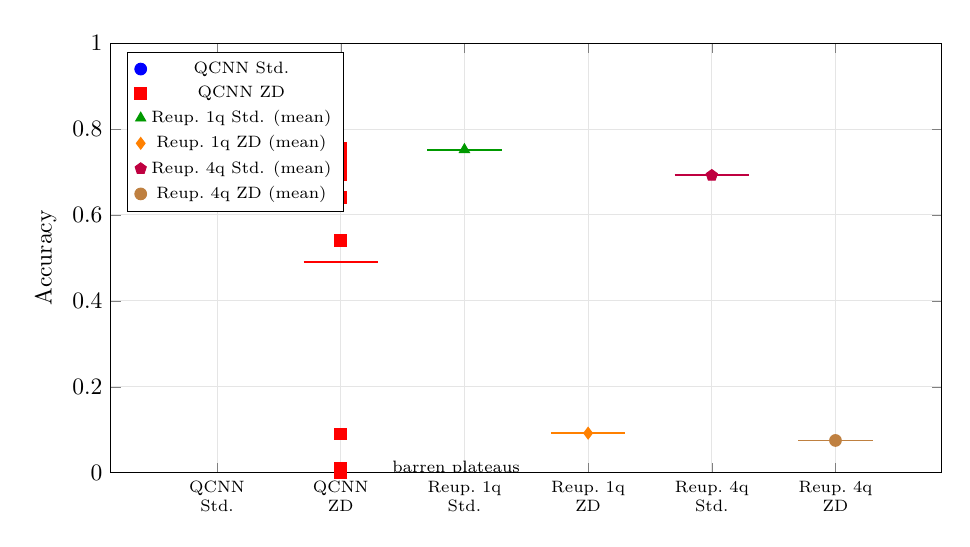
\begin{tikzpicture}[scale=0.85]
    \begin{axis}[
        ylabel={Accuracy},
        ymin=0, ymax=1.0,
        xtick={1,2,3,4,5,6},
        xticklabels={QCNN\\Std., QCNN\\ZD, Reup.~1q\\Std., Reup.~1q\\ZD, Reup.~4q\\Std., Reup.~4q\\ZD},
        x tick label style={align=center, font=\scriptsize},
        grid=major,
        grid style={gray!20},
        width=14cm, height=8cm,
        every axis plot/.append style={mark=*, mark size=2.5pt},
        legend style={at={(0.02,0.98)}, anchor=north west, font=\scriptsize},
    ]

    % QCNN Standard - 10 seeds
    \addplot[only marks, blue, mark=*] coordinates {
        (1, 0.720) (1, 0.675) (1, 0.625) (1, 0.685) (1, 0.680)
        (1, 0.690) (1, 0.665) (1, 0.680) (1, 0.660) (1, 0.710)
    };
    \addplot[blue, thick, no markers, forget plot] coordinates {(0.7, 0.679) (1.3, 0.679)};

    % QCNN Zero-day - 10 seeds
    \addplot[only marks, red, mark=square*] coordinates {
        (2, 0.755) (2, 0.640) (2, 0.010) (2, 0.730) (2, 0.695)
        (2, 0.000) (2, 0.090) (2, 0.710) (2, 0.730) (2, 0.540)
    };
    \addplot[red, thick, no markers, forget plot] coordinates {(1.7, 0.490) (2.3, 0.490)};

    % Reup 1q Standard - mean only (tightly clustered, std 0.039)
    \addplot[only marks, green!60!black, mark=triangle*] coordinates {(3, 0.752)};
    \addplot[green!60!black, thick, no markers, forget plot] coordinates {(2.7, 0.752) (3.3, 0.752)};

    % Reup 1q Zero-day
    \addplot[only marks, orange, mark=diamond*] coordinates {(4, 0.092)};
    \addplot[orange, thick, no markers, forget plot] coordinates {(3.7, 0.092) (4.3, 0.092)};

    % Reup 4q Standard
    \addplot[only marks, purple, mark=pentagon*] coordinates {(5, 0.692)};
    \addplot[purple, thick, no markers, forget plot] coordinates {(4.7, 0.692) (5.3, 0.692)};

    % Reup 4q Zero-day
    \addplot[only marks, brown, mark=otimes*] coordinates {(6, 0.075)};
    \addplot[brown, thick, no markers, forget plot] coordinates {(5.7, 0.075) (6.3, 0.075)};

    \node[black, font=\scriptsize, anchor=west] at (2.35, 0.010) {barren plateaus};

    \legend{QCNN Std., QCNN ZD, Reup.~1q Std. (mean), Reup.~1q ZD (mean), Reup.~4q Std. (mean), Reup.~4q ZD (mean)}
    \end{axis}
\end{tikzpicture}
\caption{Accuracy distribution across 10~random initialization seeds for each quantum model and task (500~samples, 100~epochs). QCNN points are individual seeds; re-uploading is shown as a single mean marker because its per-seed values are tightly clustered (standard deviations 0.011--0.039). The QCNN zero-day task exhibits three barren-plateau collapses at $\leq 9\%$, while seven seeds achieve 54--76\%. All other model--task combinations are stable across seeds.}
\label{fig:seed_box}
\end{figure}

% ---- Quantum Circuit Diagrams ----

\section{Quantum Circuit Architectures}
\label{app:circuits}

Figure~\ref{fig:qcnn_circuit} illustrates the QCNN architecture used in this work. The circuit operates on 8~qubits with 3~convolutional-pooling stages, progressively reducing the number of active qubits from 8 to 1.

\begin{figure}[ht]
\centering
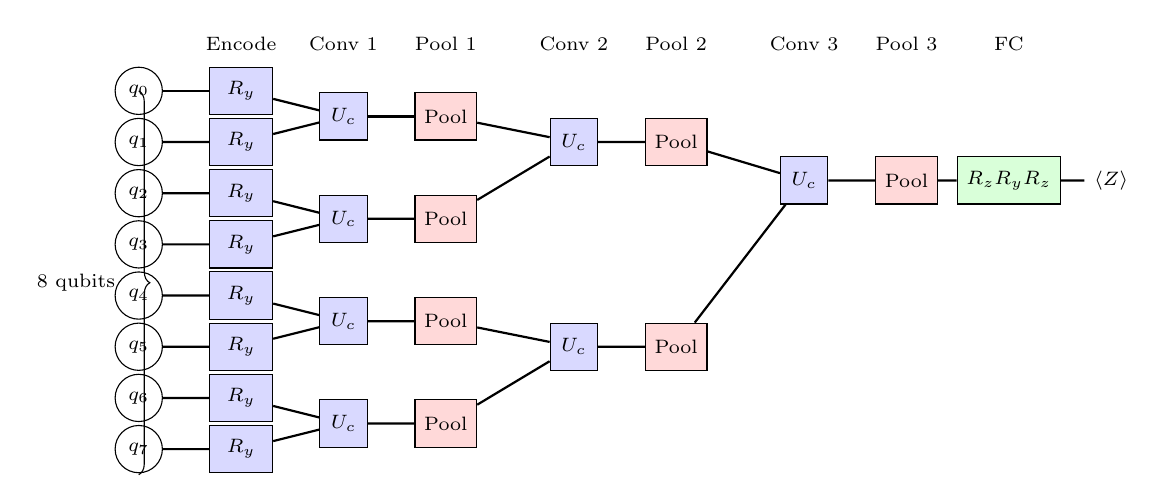
\begin{tikzpicture}[
    scale=0.65,
    qubit/.style={circle, draw, minimum size=6mm, inner sep=0pt, font=\scriptsize},
    gate/.style={rectangle, draw, fill=blue!15, minimum width=8mm, minimum height=6mm, font=\scriptsize},
    pool/.style={rectangle, draw, fill=red!15, minimum width=8mm, minimum height=6mm, font=\scriptsize},
    fc/.style={rectangle, draw, fill=green!15, minimum width=8mm, minimum height=6mm, font=\scriptsize},
    wire/.style={thick},
]
    % Qubits
    \foreach \i in {0,...,7} {
        \node[qubit] (q\i) at (0, -\i*1.0) {$q_{\i}$};
    }

    % Angle encoding
    \foreach \i in {0,...,7} {
        \node[gate] (enc\i) at (2, -\i*1.0) {$R_y$};
        \draw[wire] (q\i) -- (enc\i);
    }
    \node[font=\scriptsize, above] at (2, 0.6) {Encode};

    % Conv layer 1 (8 qubits)
    \foreach \i/\j in {0/1, 2/3, 4/5, 6/7} {
        \node[gate, minimum width=6mm] (c1\i) at (4, {-(\i+\j)/2*1.0}) {$U_c$};
        \draw[wire] (enc\i) -- (c1\i);
        \draw[wire] (enc\j) -- (c1\i);
    }
    \node[font=\scriptsize, above] at (4, 0.6) {Conv~1};

    % Pool layer 1 (8 -> 4)
    \foreach \i/\j in {0/1, 2/3, 4/5, 6/7} {
        \node[pool, minimum width=6mm] (p1\i) at (6, {-(\i+\j)/2*1.0}) {Pool};
        \draw[wire] (c1\i) -- (p1\i);
    }
    \node[font=\scriptsize, above] at (6, 0.6) {Pool~1};

    % Conv layer 2 (4 qubits)
    \foreach \i/\j in {0/2, 4/6} {
        \node[gate, minimum width=6mm] (c2\i) at (8.5, {-(\i+\j)/2*1.0}) {$U_c$};
        \draw[wire] (p1\i) -- (c2\i);
        \draw[wire] (p1\j) -- (c2\i);
    }
    \node[font=\scriptsize, above] at (8.5, 0.6) {Conv~2};

    % Pool layer 2 (4 -> 2)
    \foreach \i/\j in {0/2, 4/6} {
        \node[pool, minimum width=6mm] (p2\i) at (10.5, {-(\i+\j)/2*1.0}) {Pool};
        \draw[wire] (c2\i) -- (p2\i);
    }
    \node[font=\scriptsize, above] at (10.5, 0.6) {Pool~2};

    % Conv layer 3 (2 qubits)
    \node[gate, minimum width=6mm] (c3) at (13, -1.75) {$U_c$};
    \draw[wire] (p20) -- (c3);
    \draw[wire] (p24) -- (c3);
    \node[font=\scriptsize, above] at (13, 0.6) {Conv~3};

    % Pool layer 3 (2 -> 1)
    \node[pool, minimum width=6mm] (p3) at (15, -1.75) {Pool};
    \draw[wire] (c3) -- (p3);
    \node[font=\scriptsize, above] at (15, 0.6) {Pool~3};

    % FC layer
    \node[fc, minimum width=6mm] (fc) at (17, -1.75) {$R_z R_y R_z$};
    \draw[wire] (p3) -- (fc);
    \node[font=\scriptsize, above] at (17, 0.6) {FC};

    % Measurement
    \node[font=\scriptsize] (meas) at (19, -1.75) {$\langle Z \rangle$};
    \draw[wire] (fc) -- (meas);

    % Dimension labels
    \draw[decorate, decoration={brace, amplitude=4pt, mirror}] (0, -7.5) -- (0, 0.0)
        node[midway, left=5pt, font=\scriptsize] {8 qubits};
\end{tikzpicture}
\caption{QCNN architecture ($8 \to 4 \to 2 \to 1$ qubits). Input features are encoded via $R_y$ rotations. Three convolutional-pooling stages hierarchically reduce the circuit width. Each convolutional unitary $U_c$ applies 6~parameterized rotations; each pooling layer uses CRZ--CRY (2~parameters) to transfer information before discarding one qubit. A final $R_z R_y R_z$ layer on the remaining qubit produces the output $\langle Z \rangle \in [-1, +1]$. Total: 27~parameters per binary classifier.}
\label{fig:qcnn_circuit}
\end{figure}

Figure~\ref{fig:reup_circuit} illustrates the single-qubit data re-uploading circuit.

\begin{figure}[ht]
\centering
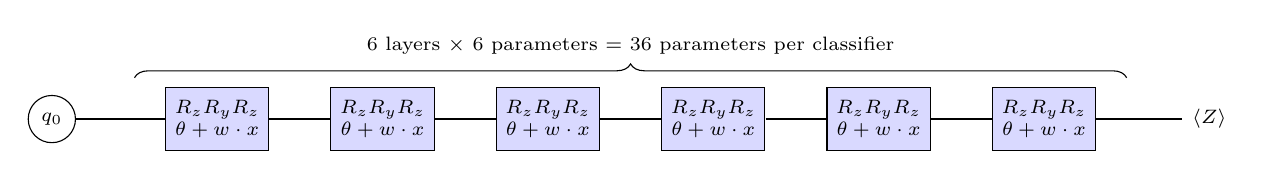
\begin{tikzpicture}[
    scale=0.75,
    qubit/.style={circle, draw, minimum size=6mm, inner sep=0pt, font=\scriptsize},
    gate/.style={rectangle, draw, fill=blue!15, minimum width=10mm, minimum height=8mm, font=\scriptsize, align=center},
    wire/.style={thick},
]
    % Single qubit
    \node[qubit] (q) at (0, 0) {$q_0$};

    % Layers
    \foreach \l [count=\i from 1] in {1,2,3,4,5,6} {
        \pgfmathsetmacro{\x}{\i * 2.8}
        \node[gate] (layer\l) at (\x, 0) {$R_z R_y R_z$\\$\theta + w \cdot x$};
        \ifnum\i=1
            \draw[wire] (q) -- (layer\l);
        \else
            \pgfmathtruncatemacro{\prev}{\l-1}
            \draw[wire] (layer\prev) -- (layer\l);
        \fi
    }

    % Measurement
    \node[font=\scriptsize] (meas) at (19.6, 0) {$\langle Z \rangle$};
    \draw[wire] (layer6) -- (meas);

    % Brace
    \draw[decorate, decoration={brace, amplitude=5pt}] (2.8-1.4, 0.7) -- (16.8+1.4, 0.7)
        node[midway, above=5pt, font=\scriptsize] {6 layers $\times$ 6 parameters = 36 parameters per classifier};

\end{tikzpicture}
\caption{Single-qubit data re-uploading circuit (6~layers). Each layer applies parameterized $R_z R_y R_z$ rotations where the rotation angles are $\theta_j^{(l)} + w_j^{(l)} \cdot x_{f(j,l)}$, combining trainable weights with input features that cycle across layers. The same qubit is reused across all layers, enabling a single qubit to learn complex decision boundaries. Total: 36~parameters per binary classifier.}
\label{fig:reup_circuit}
\end{figure}

Figure~\ref{fig:reup_multi_circuit} shows the multi-qubit variant used in this work: 4~qubits with 3~re-uploading layers and nearest-neighbor CZ entanglement between layers.

\begin{figure}[ht]
\centering
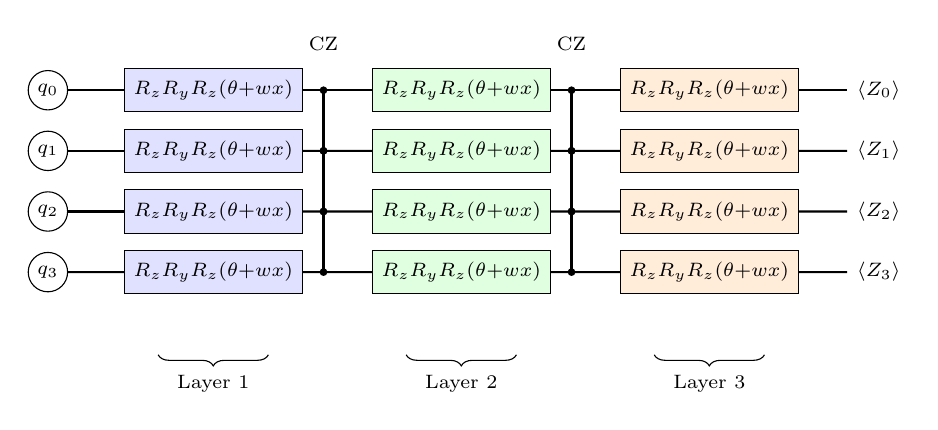
\begin{tikzpicture}[
    scale=0.7,
    qubit/.style={circle, draw, minimum size=5mm, inner sep=0pt, font=\scriptsize},
    gate/.style={rectangle, draw, fill=blue!12, minimum width=16mm, minimum height=5.5mm, font=\scriptsize, align=center},
    wire/.style={thick},
]
    % Qubit labels
    \foreach \q in {0,1,2,3} {
        \node[qubit] (q\q) at (0, -\q*1.1) {$q_\q$};
    }

    % Layer 1 gates
    \foreach \q in {0,1,2,3} {
        \node[gate] (l1q\q) at (3, -\q*1.1) {$R_z R_y R_z(\theta{+}wx)$};
        \draw[wire] (q\q) -- (l1q\q);
    }

    % CZ entanglement 1
    \foreach \q in {0,1,2} {
        \pgfmathtruncatemacro{\qq}{\q+1}
        \draw[thick] (5, -\q*1.1) -- (5, -\qq*1.1);
        \fill (5, -\q*1.1) circle (0.07);
        \fill (5, -\qq*1.1) circle (0.07);
    }
    \node[above, font=\scriptsize] at (5, 0.55) {CZ};
    \foreach \q in {0,1,2,3} {
        \draw[wire] (l1q\q) -- (5, -\q*1.1);
    }

    % Layer 2 gates
    \foreach \q in {0,1,2,3} {
        \node[gate, fill=green!12] (l2q\q) at (7.5, -\q*1.1) {$R_z R_y R_z(\theta{+}wx)$};
        \draw[wire] (5, -\q*1.1) -- (l2q\q);
    }

    % CZ entanglement 2
    \foreach \q in {0,1,2} {
        \pgfmathtruncatemacro{\qq}{\q+1}
        \draw[thick] (9.5, -\q*1.1) -- (9.5, -\qq*1.1);
        \fill (9.5, -\q*1.1) circle (0.07);
        \fill (9.5, -\qq*1.1) circle (0.07);
    }
    \node[above, font=\scriptsize] at (9.5, 0.55) {CZ};
    \foreach \q in {0,1,2,3} {
        \draw[wire] (l2q\q) -- (9.5, -\q*1.1);
    }

    % Layer 3 gates
    \foreach \q in {0,1,2,3} {
        \node[gate, fill=orange!15] (l3q\q) at (12, -\q*1.1) {$R_z R_y R_z(\theta{+}wx)$};
        \draw[wire] (9.5, -\q*1.1) -- (l3q\q);
    }

    % Final CZ + measurement
    \foreach \q in {0,1,2,3} {
        \draw[wire] (l3q\q) -- (14.5, -\q*1.1);
        \node[right, font=\scriptsize] at (14.5, -\q*1.1) {$\langle Z_{\q} \rangle$};
    }

    % Layer braces below
    \draw[decorate, decoration={brace, amplitude=4pt, mirror}] (2.0, -4.8) -- (4.0, -4.8)
        node[midway, below=4pt, font=\scriptsize] {Layer~1};
    \draw[decorate, decoration={brace, amplitude=4pt, mirror}] (6.5, -4.8) -- (8.5, -4.8)
        node[midway, below=4pt, font=\scriptsize] {Layer~2};
    \draw[decorate, decoration={brace, amplitude=4pt, mirror}] (11.0, -4.8) -- (13.0, -4.8)
        node[midway, below=4pt, font=\scriptsize] {Layer~3};
\end{tikzpicture}
\caption{Multi-qubit data re-uploading circuit (4~qubits, 3~layers). Each qubit independently applies parameterized $R_z R_y R_z$ rotations that mix input data $\mathbf{x}$ with trainable weights, with nearest-neighbor CZ gates entangling the qubits between layers. The final output is the average of the per-qubit $\langle Z \rangle$ measurements, expressed as a single Hamiltonian measurement $\langle H \rangle = \tfrac{1}{n}\sum_q Z_q$. Total: $6 \times 4 \times 3 = 72$~parameters per binary classifier.}
\label{fig:reup_multi_circuit}
\end{figure}
